\documentclass[dvipdfmx]{article}
\usepackage[dvipdfmx]{graphicx}
\usepackage{amsmath, amssymb}
\usepackage{mathtools}
\usepackage{here}

\begin{document}
\title{Weekly Report}
\author{Riku Gondow}
\maketitle

\section{Progress}
\begin{itemize}
    \item Implement LSTM-CNN Ensemble method\cite{lstm}
    \begin{itemize}
        \item I'm still implementing LSTM and CNN based on the paper, and it worked for the sample data.
    \end{itemize}
\end{itemize}

\begin{figure}[H]
\begin{center}
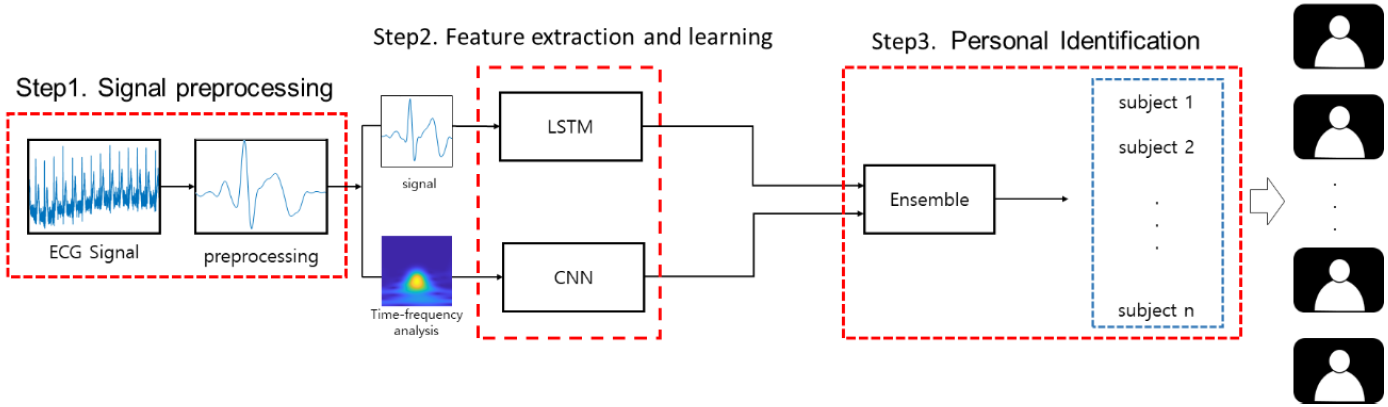
\includegraphics[width=\linewidth]{./img/LSTM-CNN.png}
\end{center}
\caption{LSTM-CNN Ensemble method}
\end{figure}

\section{Next Plan}
\begin{itemize}
    \item Evaluate LSTM-CNN Ensemble method on 30-subjects dataset.
\end{itemize}

\begin{thebibliography}{99}
\bibitem{lstm} Lee, Jin-A., and Keun-Chang Kwak. "Personal Identification Using an Ensemble Approach of 1D-LSTM and 2D-CNN with Electrocardiogram Signals." Applied Sciences 12.5 2022: 2692.
\end{thebibliography}

\end{document}